\section{Dataset Preparation}
We employ Freebase to automatically annotate text in Wikipedia. We regard a sentence as a positive one when it suggests an occurrence of event, or otherwise a negative sentence. For example, S1 and S2 are positive sentences and their arguments are in italics and underlined, while S3 and S4 are negative sentences. The event structures of S1 and S2 are illustrated in Figure~\ref{fig:3}.

\begin{quote}
	\textbf{S1}: \underline{\emph{Remedy Corp}} was sold to \underline{\emph{BMC Software}} as the \underline{\emph{Service Management Business}} Unit in \underline{\emph{2004}}.
\end{quote}
\begin{quote}
	\textbf{S2}: \underline{\emph{Microsoft}} spent \$6.3 billion buying online display advertising company \underline{\emph{aQuantive}} in \underline{\emph{2007}}.
\end{quote}
\begin{quote}
	\textbf{S3}: Microsoft hopes aQuantive's Brian McAndrews can outfox Google.
\end{quote}
\begin{quote}
	\textbf{S4}: On April 29th, Elizabeth II and Prince Philip witnessed the marriage of Prince William.
\end{quote}

\subsection{Freebase}
Freebase\cite{bollacker2008freebase} is a collaborative structured knowledge base which be divided into three layers: \emph{domain}, \emph{type} and \emph{instance}. \emph{Instances} are entries in Freebase, and are related to real-world entities like people and places. \emph{Types} are different perspectives of \emph{instances}. \textbf{\emph{Compound Value Type}} (CVT) is a special type in Freebase to represent complex structured data where each instance consists of multiple \textbf{\emph{properties}}. Some of the CVT schemas are highly alike to event structures where CVT properties can be treat as event arguments. For example, in Figure~\ref{fig:3}, \emph{business.acquisition} is a CVT whose properties are \emph{company\_acquired}, \emph{acquiring\_company}, \emph{date} and \emph{divisions\_formed}. These properties can also be used to represent participants and attributes in events extracted from S1 and S2.

We use the Freebase version of Berant et al. \shortcite{berant2013semantic}, containing 1010 CVTs. After filtering out CVTs that describe the structures of the Freebase or are irrelevant to event extraction (e.g., \emph{food.recipe\_ingredient}), we select 24 types of CVTs with around 280 million instances.

\begin{figure}[h]
	\centering
	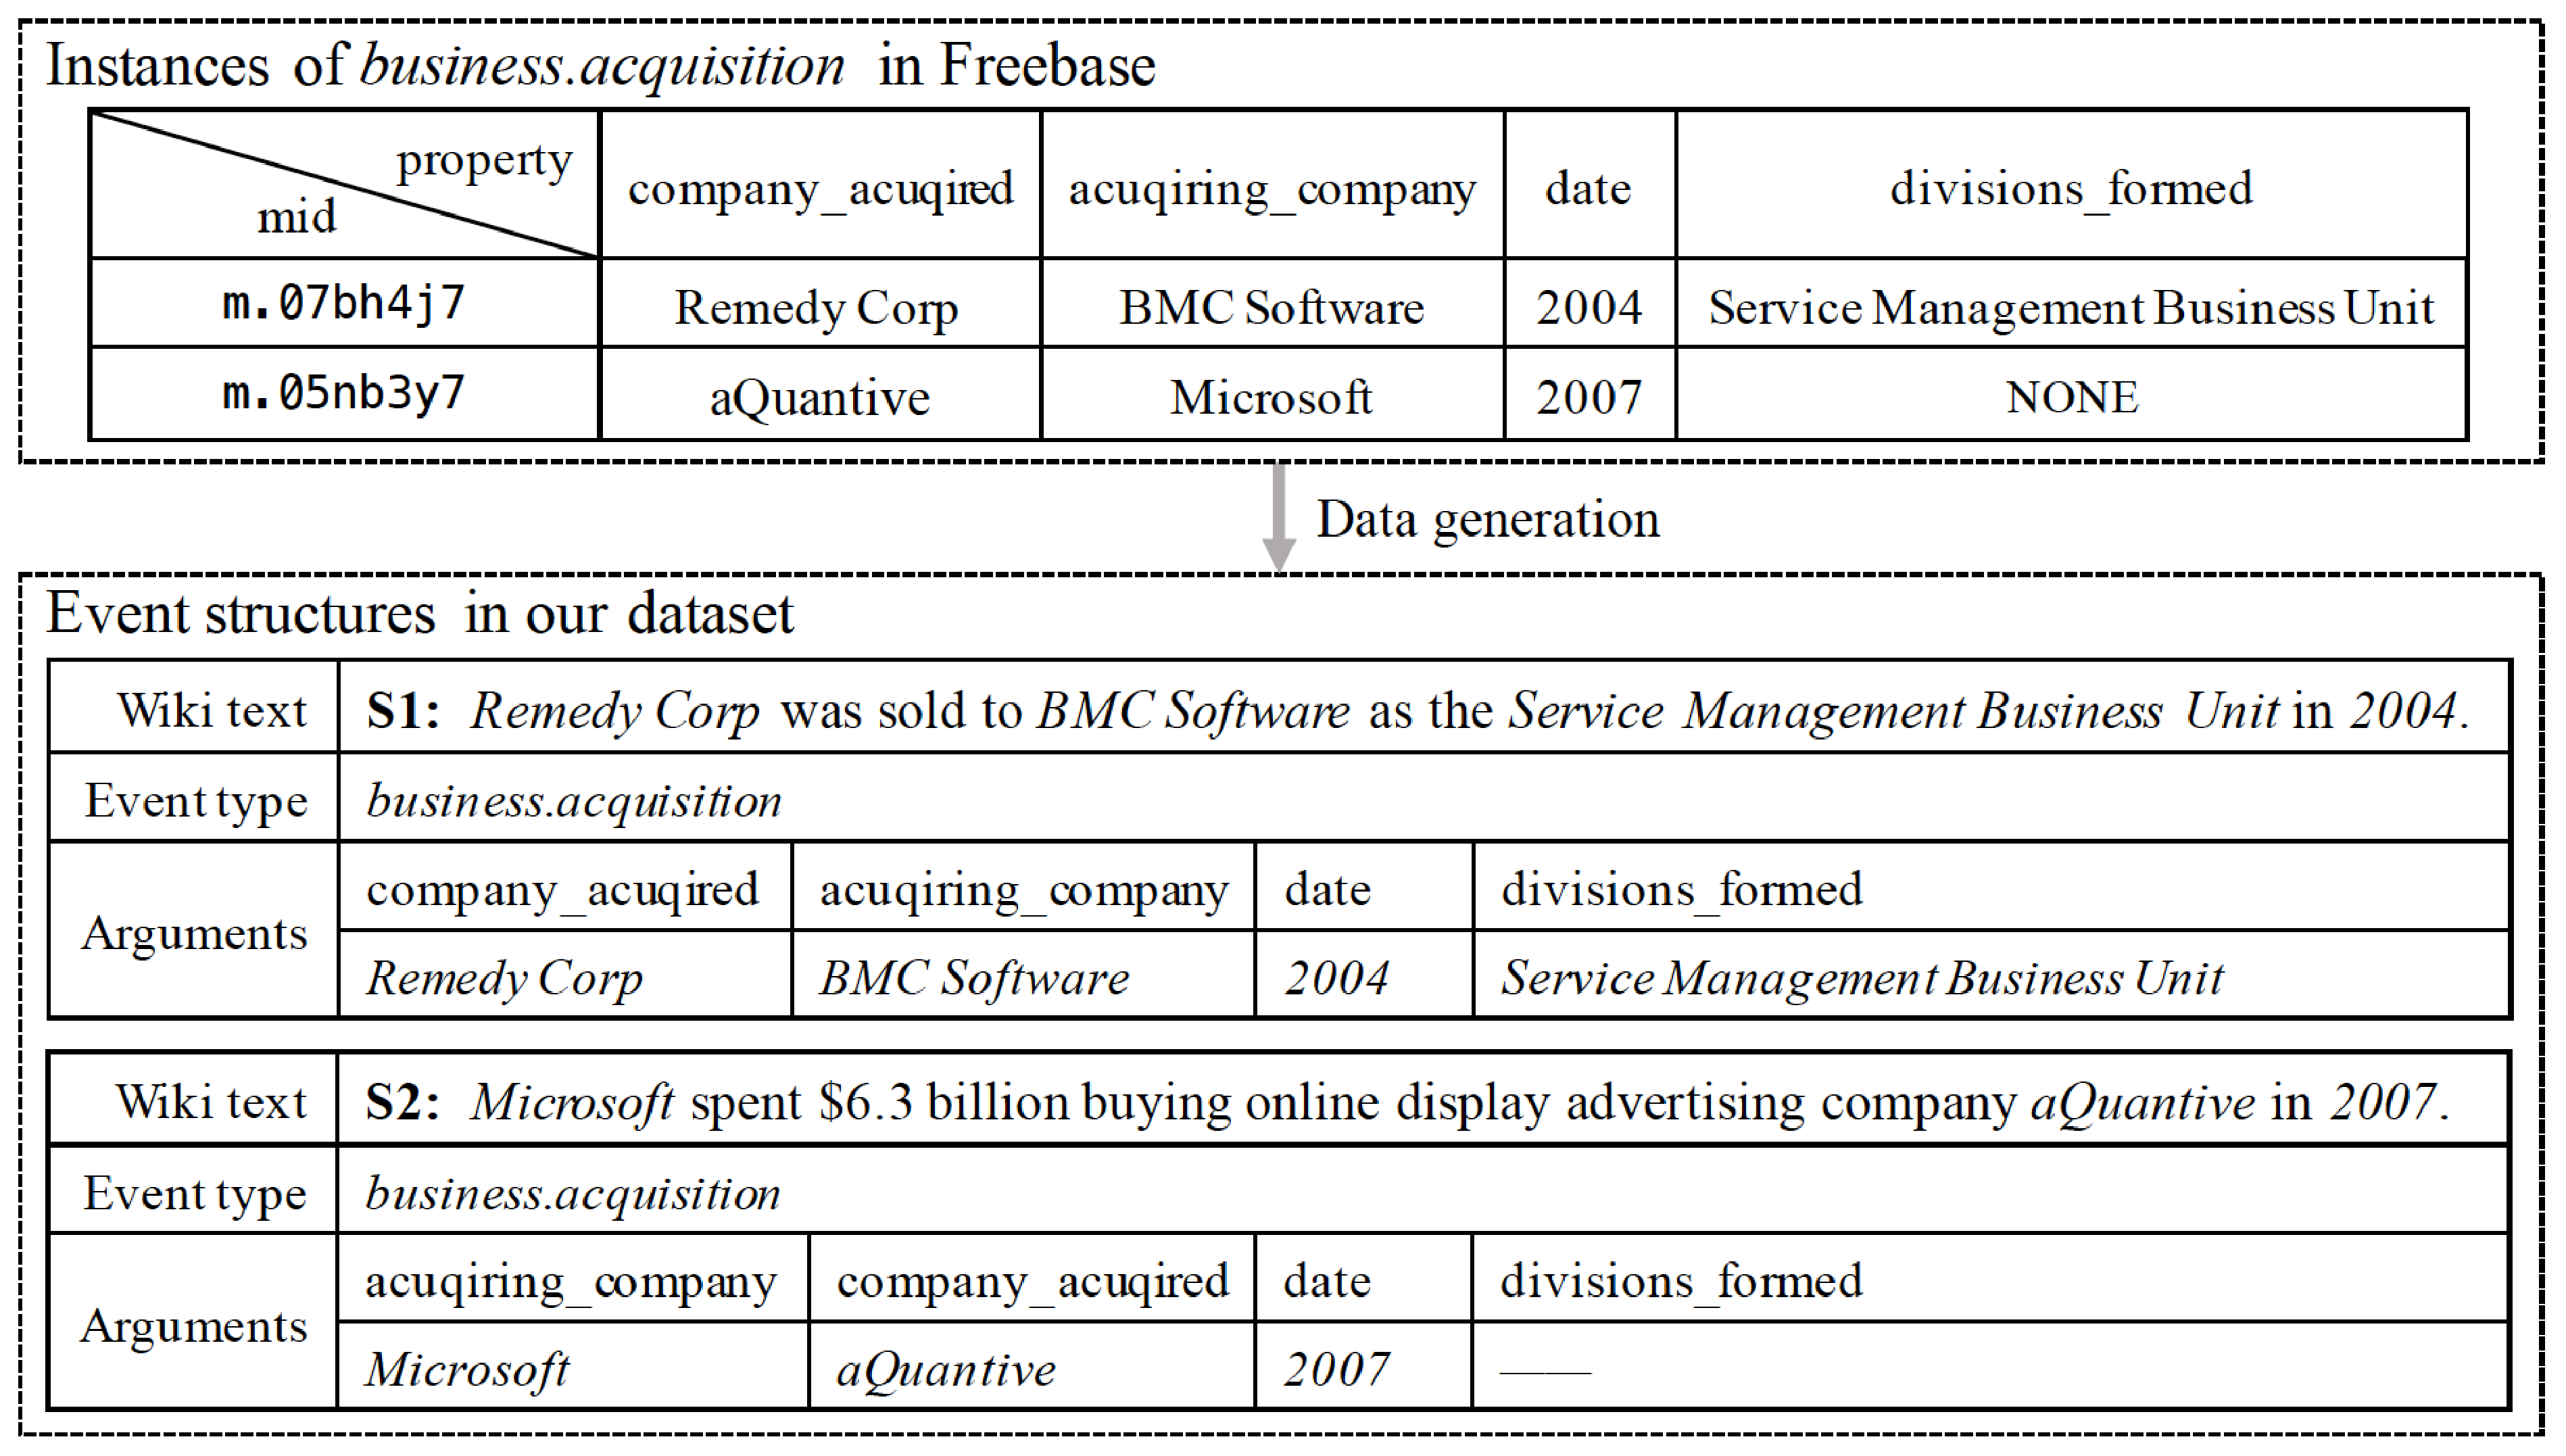
\includegraphics[width=.48\textwidth]{temp}
	\caption{Examples of CVT instances in Freebase, and labeled sentences in our dataset. \emph{Company\_acuqired}, \emph{acquiring\_company} and \emph{date} are key arguments in \emph{business.acquisition}. \label{fig:3}}
\end{figure}

\subsection{Data Generation\label{datagen}}
\subsubsection{H1: Positive sentences should contain all properties}
This hypothesis indicates that if a sentence has all properties of a CVT, it is more likely to be a positive sentence. We regard the CVT as event type and extract words and phrases that match the properties of a CVT instance as involved arguments. For example, S1 contains all the properties of instance $m.07bh4j7$ whose type is \emph{business.acquisition}, thus we consider S1 as a positive sentence which implies an event about \emph{business.acquisition}, and \emph{BMC Software}, \emph{Remedy Corp}, \emph{Service Management Business Unit} and \emph{2004} should be labeled as the arguments that play the role of \emph{acquiring\_company}, \emph{company\_acquired}, \emph{divisions\_formed}, \emph{date}, respectively.

However, in practice, we realize that \emph{H1} is too strict that excludes a great many positive sentences like S2. 

\subsubsection{H2: Positive sentences should contain all key properties}
This hypothesis is an extension of \emph{H1}, which relaxes ``all properties'' constraint to ``key properties''. We define the CVT property that plays an important part in its CVT structure and helps to distinguish with other CVT as \textbf{key property}. And \textbf{key argument} is the word/phrase that matches a key property of a CVT instance. For example, \emph{company\_acquired} and \emph{acquiring\_company} are the key properties of CVT \emph{business.acquisition}, and with this relaxation, positive sentences like S2 need not contain all properties, but only key properties instead.

The importance of a property $pro$ (e.g., \emph{date}) to its CVT $cvt$ (e.g., \emph{business.acquisition}) can be defined as follows:
\begin{equation}
	degree_{cvt, pro} = log \frac{count(cvt, pro)}{count(cvt) \times count(pro)} 
\end{equation}
where $count(cvt)$ is the number of all $cvt$ instances, $count(pro)$ is the number of $pro$ among all CVTs, and $count(cvt, pro)$ is the number of $cvt$ instances that contain the property $pro$.

\subsubsection{H3: Key properties should include time property}
We discover that for many CVTs, their key properties do not take into account time property. However, ignoring time property will produce a large number of negative sentences like S3. It does not express an explicit event about \emph{business.accquisition} while contain all key properties of an instance, resulting in mistaking \emph{Microsoft} for \emph{acquiring\_company}, and \emph{aQuantive} for \emph{company\_acquired}. By adding \emph{date} to the set of key properties, S3 will be filtered. Therefore, we choose the time property which achieves the highest importance value as a supplementary key property. 

\subsubsection{H4: Positive sentences should contain key properties with close syntactic distance}
We introduce another factor, syntactic distance, to annotate positive sentences. Intuitively, two arguments participant in the same event are likely to have close syntactic distance. This factor is effective to eliminate negative sentences, such as S4. The syntactic distance can be measured by the distance of two words in dependency parsing tree. We set the maximum distance between two key arguments as 2, denoting that, for a candidate sentence, if a pair of key arguments violates this constraint, it is supposed to be negative. Given the dependency parsing tree in Figure~\ref{fig:2}, S4 is negative because the distance between \emph{Prince Philip} and \emph{marriage} is 3.

\begin{figure}
	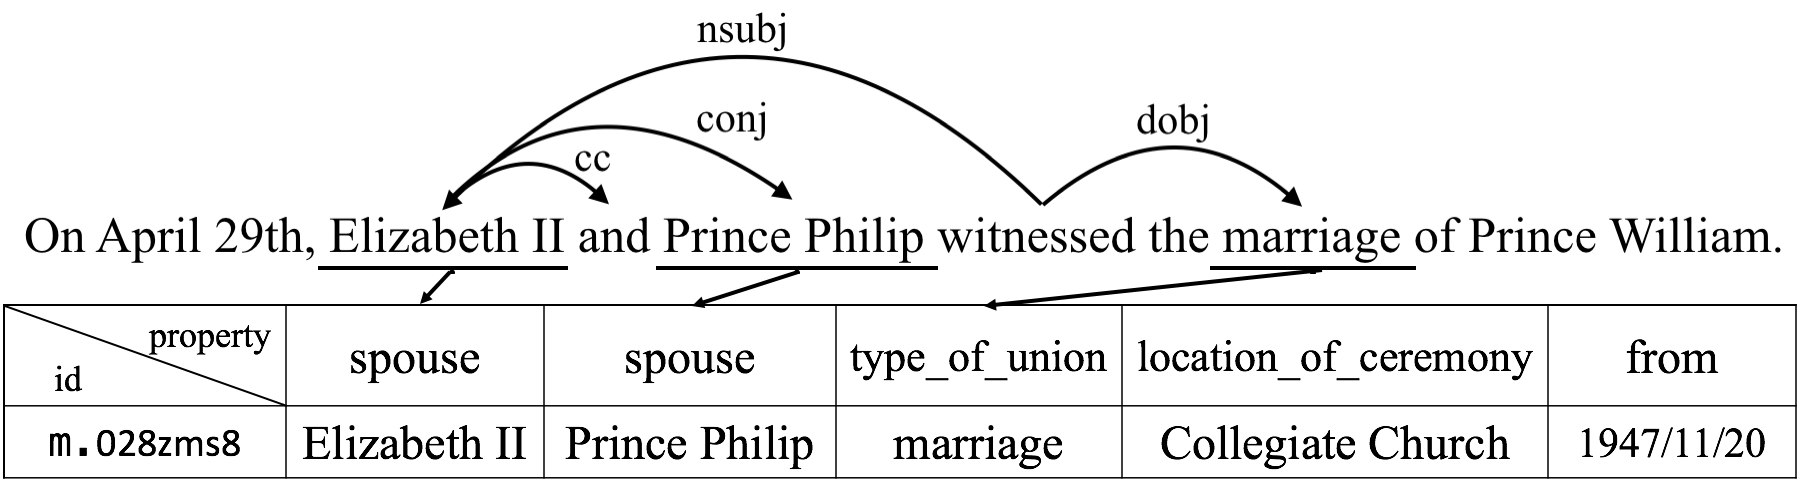
\includegraphics[width=.48\textwidth]{deppath}
	\caption{An illustration of dependency parse tree of S4. \label{fig:2}}
\end{figure}

We conduct a manual evaluation on the quantity and quality of  datasets generated by different hypotheses (see Section~\ref{sec:evalhypo}), and utilize the combinations of hypothesis \emph{H3} and \emph{H4} as the final strategy.